%https://chem.libretexts.org/Bookshelves/Physical_and_Theoretical_Chemistry_Textbook_Maps/Supplemental_Modules_(Physical_and_Theoretical_Chemistry)/Spectroscopy/Magnetic_Resonance_Spectroscopies/Electron_Paramagnetic_Resonance/EPR_-_Interpretation

\documentclass{article}
\usepackage[utf8]{inputenc}
\usepackage{blindtext}
\usepackage{graphicx}
\usepackage{amsmath}
\usepackage{csvsimple}
\usepackage{pdfpages}
\usepackage{hyperref}
\usepackage{gensymb}

\begin{document}
\begin{center}
\textbf{\Huge{University of South Bohemia}}\\
\vspace{50px}
\textbf{\Large{Faculty of Science}} \\
\vspace{30px}
\includegraphics[width=120px]{~/school/logo.png} \\
\vspace{30px}
\textbf{\large{Praktika IV}}
\vspace{20px}
\\
\vspace{20px}
\large{Frank-Hertzův experiment} \\
\vspace{60px}
\end{center}
\begin{flushleft}
Datum: 5.12.2023 \\
Jmeno: Martin Skok \\
Obor: Fyzika \\
Hodnoceni:
\end{flushleft}
\newpage
\section{Úkoly}
\begin{itemize}
\item Změřte závislost magnetického pole na rezonanční frekvenci vzorku DPPH (radikál 2,2-difenyl-1-pikrylhydrazylu) \\
\item Určete jeho $g$ faktor.
\end{itemize}
\section{Seznam pomůcek}
Počítač, 3B-NET log, 3B-NET lab program, jednostka s cívkami a se sondou, vzorek DPPH
\section{Teorie}
EPR nebo ESP je metoda, při níž se hledají prvky s nepárovanými elektrony, neboli radikáli.
Elektrony mají několik vlastností, kterými jsou náboj, hmotnost a spin. Nezpárované elektrony můžou okupovat \\ hodnoty $m_{s} = + \frac{1}{2}$ nebo $m_{s} = - \frac{1}{2}$.
K magnetickému poli přispívá spinový magnetický moment. Interakce mezi magnetickým polem a magnetickým momentem je dána vztahem
\begin{equation}
  \Delta E = h f = g \mu_{B} B
\end{equation}
kde $g$ je faktor volného elektronu který má má hodnotu $2.002319$\\
$\mu_{b}$ Bohrův magnetron s hodnotou $9.72401\cdot 10^{-24}$
Vztah můžeme upravit a vyjádřit $g$ faktor
\begin{equation}
  g = \frac{f_{r}h}{B_{r}\mu_{B}}
\end{equation}
Magnetické pole v našem případě můžeme vyjádřit jako
\begin{equation}
  B_{r} = 3.648 U_{r}
\end{equation}
kde $U_{r}$ je rezonanční napětí cívky.
\section{Postum měření}
Sestavil jsem a zapnul obvod\\
Vložil jsem vzorek DPPH\\
Zapnul jsem počítač a spustil program 3B-NET lab\\
Nastavil jsem potřebné paratemry a spustil osciloskop\\
Nastavil jsem frekvenci na $40 MHz$ a uložil data\\
Toto jsem opakoval do frekvence kolem $80 Mhz$ po intervalech kolem $5Mz$\\
Frekvence jsem ne vždy dokázal nastavit na přesnou hodnotu, tak jsem si vždy zapsal aktualňí hodnotu frekvence\\
\section{Naměřená data}
\begin{figure}[!h]
  \hspace*{-10em}
  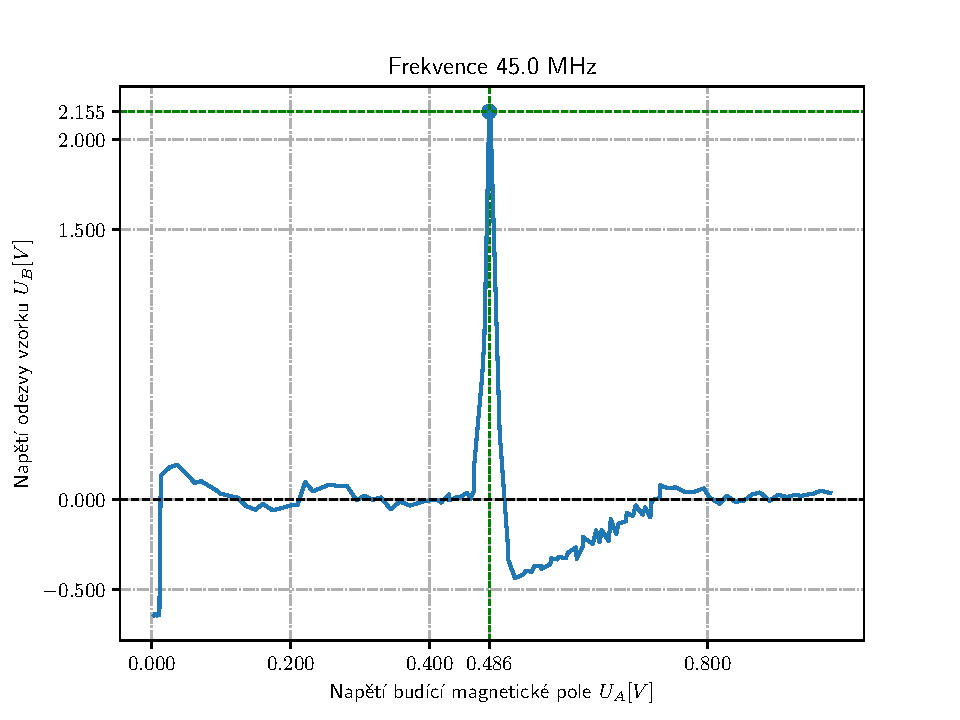
\includegraphics[scale=1.2]{figs/1.pdf}
  \caption{Graf závislosti napětí odezvy vzorku na napětím budícím magnetické pole}
\end{figure}
\clearpage
\begin{figure}[!h]
  \hspace*{-10em}
  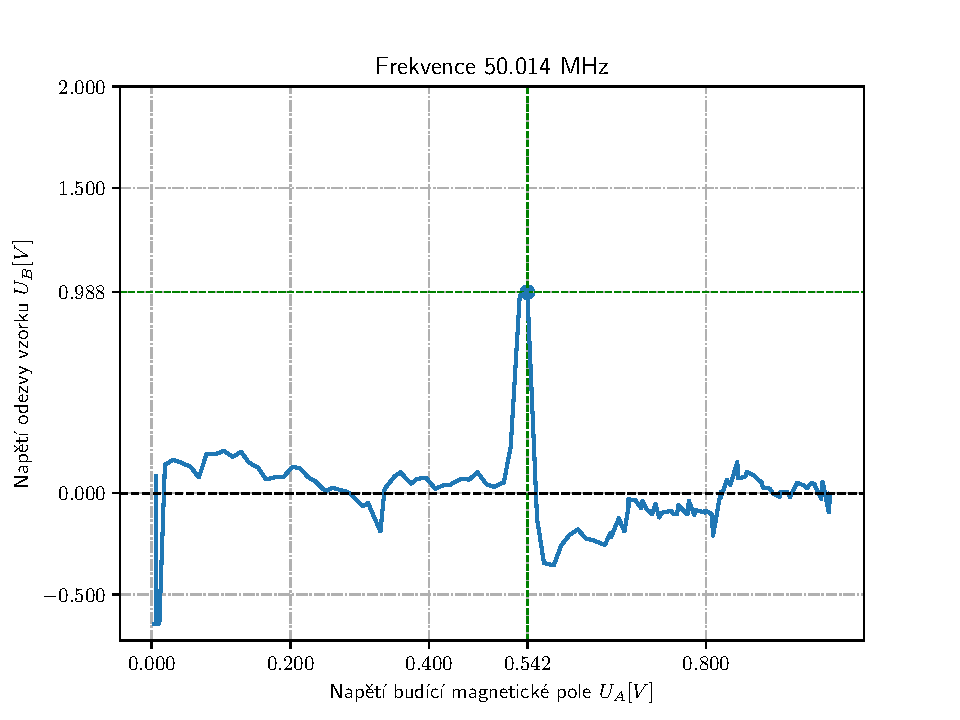
\includegraphics[scale=1.2]{figs/2.pdf}
  \caption{Graf závislosti napětí odezvy vzorku na napětím budícím magnetické pole}
\end{figure}
\clearpage
\begin{figure}[!h]
  \hspace*{-10em}
  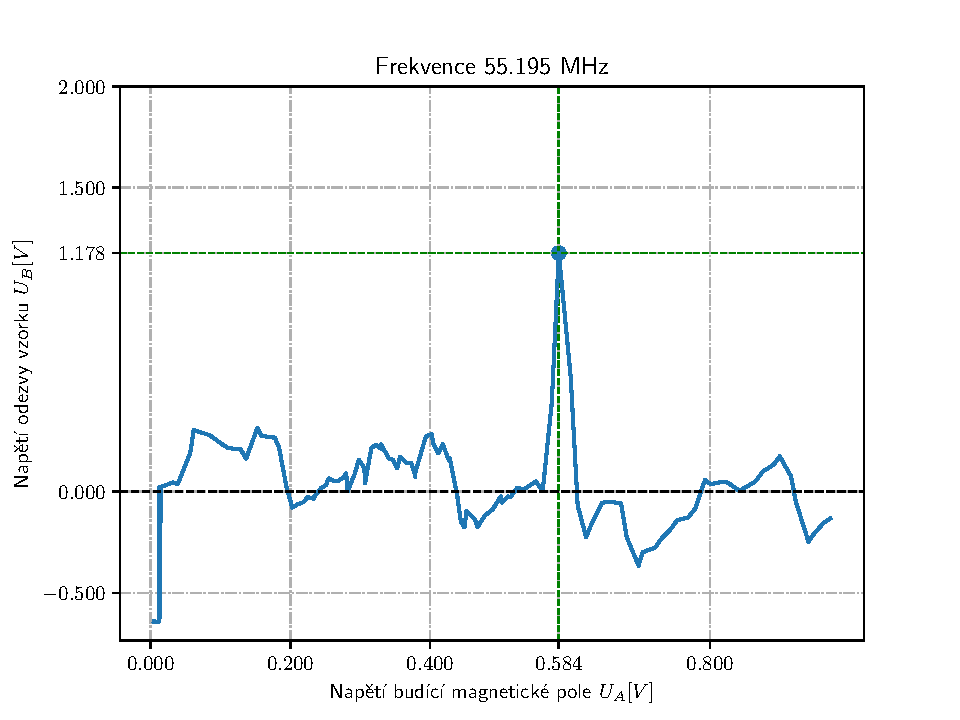
\includegraphics[scale=1.2]{figs/3.pdf}
  \caption{Graf závislosti napětí odezvy vzorku na napětím budícím magnetické pole}
\end{figure}
\clearpage
\begin{figure}[!h]
  \hspace*{-10em}
  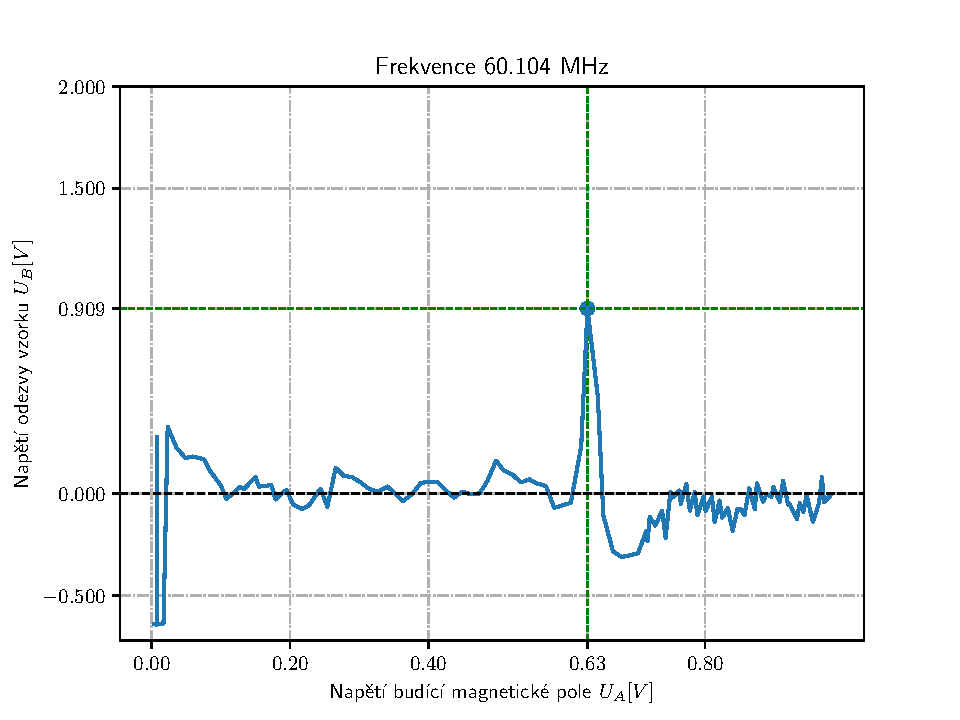
\includegraphics[scale=1.2]{figs/4.pdf}
  \caption{Graf závislosti napětí odezvy vzorku na napětím budícím magnetické pole}
\end{figure}
\clearpage
\begin{figure}[!h]
  \hspace*{-10em}
  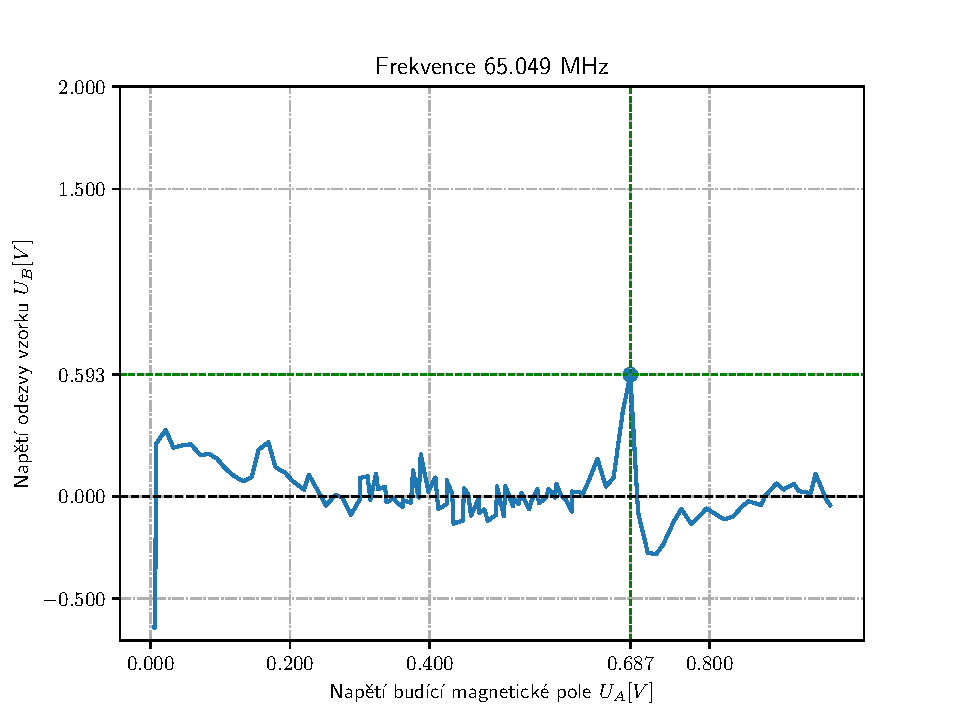
\includegraphics[scale=1.2]{figs/5.pdf}
  \caption{Graf závislosti napětí odezvy vzorku na napětím budícím magnetické pole}
\end{figure}
\clearpage
\begin{figure}[!h]
  \hspace*{-10em}
  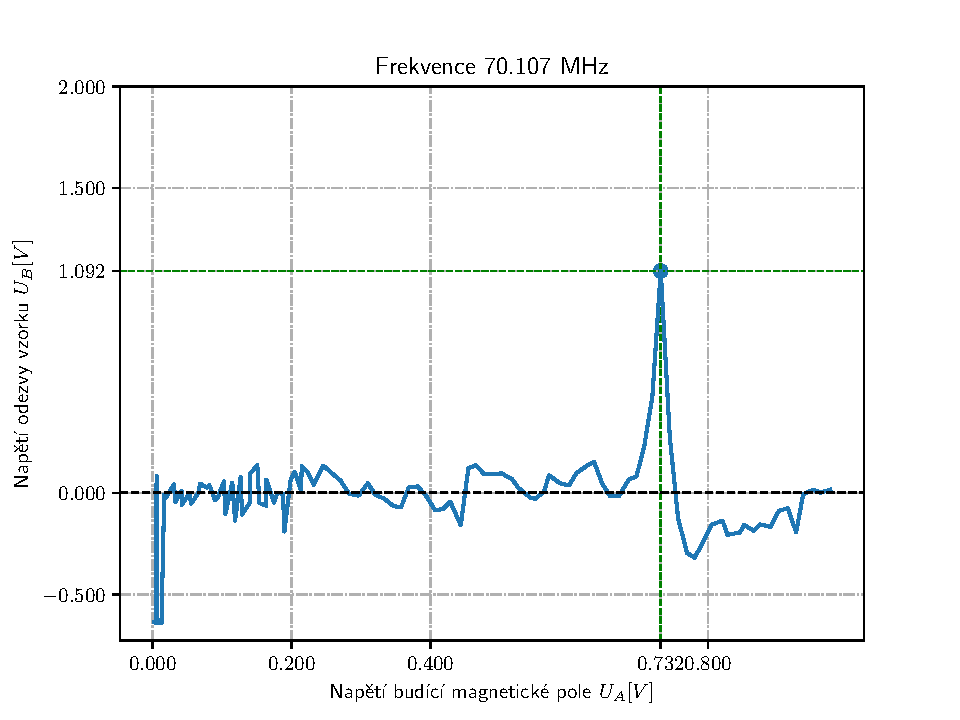
\includegraphics[scale=1.2]{figs/6.pdf}
  \caption{Graf závislosti napětí odezvy vzorku na napětím budícím magnetické pole}
\end{figure}
\clearpage
\begin{figure}[!h]
  \hspace*{-10em}
  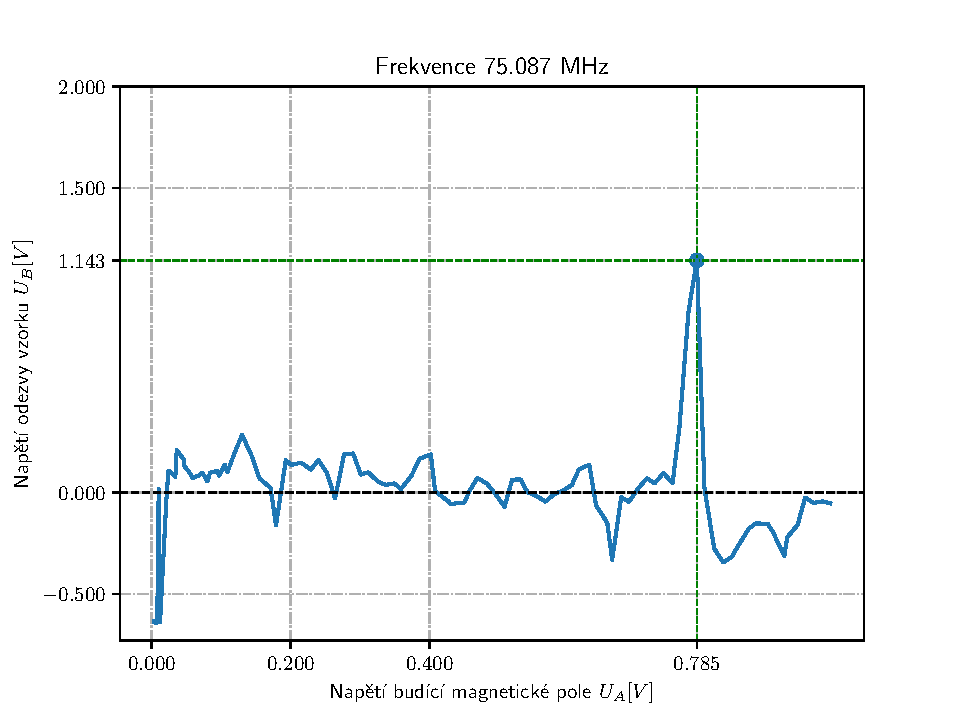
\includegraphics[scale=1.2]{figs/7.pdf}
  \caption{Graf závislosti napětí odezvy vzorku na napětím budícím magnetické pole}
\end{figure}
\clearpage
\begin{figure}[!h]
  \hspace*{-10em}
  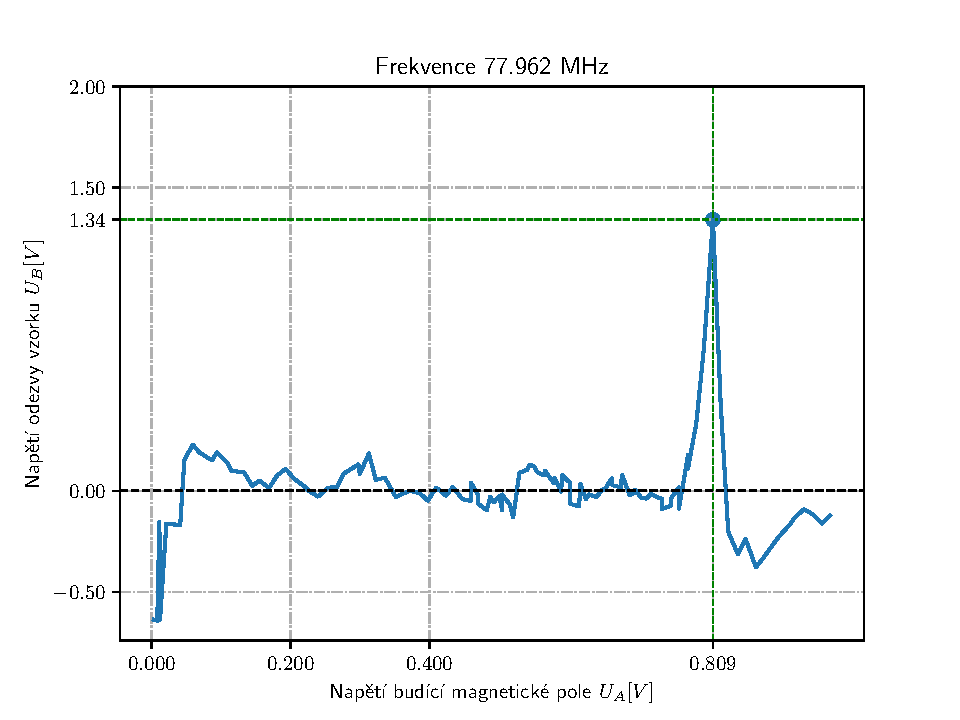
\includegraphics[scale=1.2]{figs/8.pdf}
  \caption{Graf závislosti napětí odezvy vzorku na napětím budícím magnetické pole}
\end{figure}
\newpage

\section{Zpracování dat}
\footnotesize{Tabulka 1:}\\
\large{
\csvreader[
tabular = |c|c|c|c|c|,
table head =
\hline
{index}&{$f_{r} [MHz]$}&{$U_{r} [V]$}&{$B_{r} [mT]$}&{$g$}\\
\hline
\hline,
late after line = \\\hline
]{figs/resd.csv}{}{
  \csvcoli & \csvcolii & \csvcoliii & \csvcoliv & \csvcolv}
\\
}
\vspace{1em}
\\
Hodnoty $U_{r}$ jsou hodnoty peaků na grafech. Magnetické pole $B_{r}$ jsem počítal podle vztahu \textbf{3}.\\
$g$ faktor jsem počítal podle vztahu \textbf{2}.
$$\overline{g} = \sum^{n}_{i=1}\frac{g_{i}}{n}$$
$\overline{g} = 1.8539$\\

$$\sigma_{g} = \sqrt{\frac{\sum^{n}_{i=1}(g_{i} - \overline{g})^{2}}{n-1}}$$
$\sigma_{g} = 0.029307$
\\
\vspace{1em}
\begin{figure}[H]
  \hspace*{-8em}
  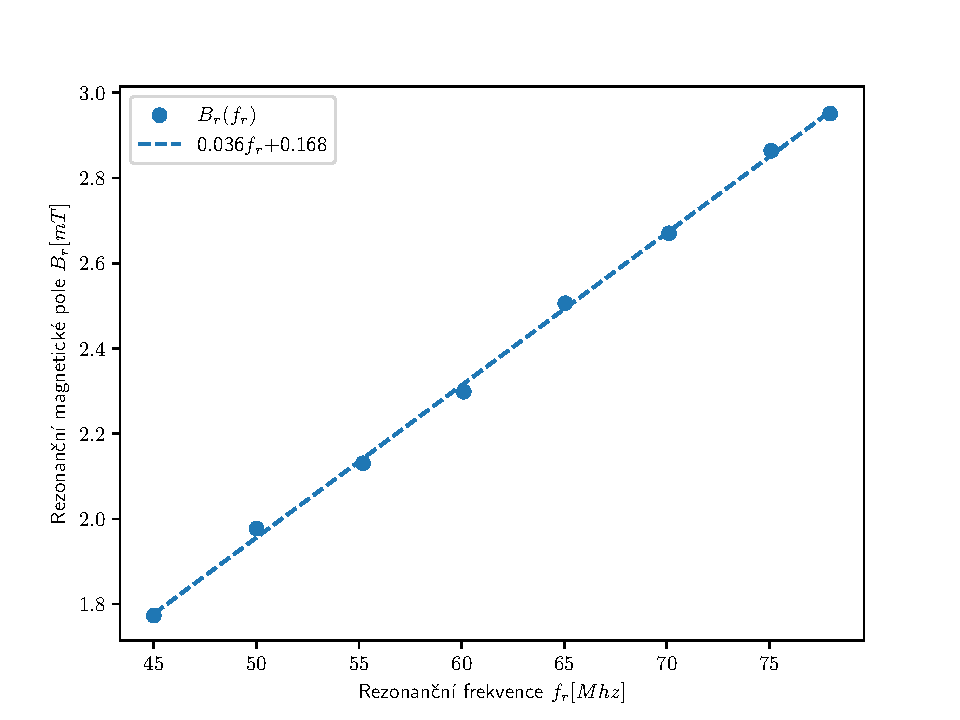
\includegraphics[scale=1]{figs/resd.pdf}
  \caption{Graf závislosti napětí odezvy vzorku na napětím budícím magnetické pole}
\end{figure}
\clearpage
\section{Diskuse}
Z měření je vidět, že se námi naměřená hodnota $g$ liší od hodnoty udavané ze zdrojů. Chyba může být způsobena špatným nastavováním hodnot nebo jino neznámou chybou, které jsem se mohl dopustit.
\section{Závěr}
$$g = 1.8539 \pm 0.0293$$
\section{Zdroje}

\url{https://chem.libretexts.org/Bookshelves/Physical_and_Theoretical_Chemistry_Textbook_Maps/Supplemental_Modules_(Physical_and_Theoretical_Chemistry)/Spectroscopy/Magnetic_Resonance_Spectroscopies/Electron_Paramagnetic_Resonance/EPR_-_Interpretation}
\end{document}
